%%%%%%%%%%%%%%%%%%%%%%%%%%%%%%%%%%%%%%%%%
% Short Sectioned Assignment LaTeX Template Version 1.0 (5/5/12)
% This template has been downloaded from: http://www.LaTeXTemplates.com
% Original author:  Frits Wenneker (http://www.howtotex.com)
% License: CC BY-NC-SA 3.0 (http://creativecommons.org/licenses/by-nc-sa/3.0/)
%%%%%%%%%%%%%%%%%%%%%%%%%%%%%%%%%%%%%%%%%

% \documentclass[paper=a4, fontsize=11pt]{scrartcl} % A4 paper and 11pt font size
\documentclass[11pt, a4paper]{book}
\usepackage[T1]{fontenc} % Use 8-bit encoding that has 256 glyphs
\usepackage[utf8]{inputenc}
% \usepackage{fourier} % Use the Adobe Utopia font for the document - comment this line to return to the LaTeX default
\usepackage{listings} % para insertar código con formato similar al editor
\usepackage[spanish, es-tabla]{babel} % Selecciona el español para palabras introducidas automáticamente, p.ej. "septiembre" en la fecha y especifica que se use la palabra Tabla en vez de Cuadro
\usepackage{url} % ,href} %para incluir URLs e hipervínculos dentro del texto (aunque hay que instalar href)
\usepackage{graphics,graphicx, float} %para incluir imágenes y colocarlas
\usepackage[gen]{eurosym} %para incluir el símbolo del euro
%\usepackage{cite} %para incluir citas del archivo <nombre>.bib
\usepackage[style=apa, backend=biber]{biblatex}
\addbibresource{bibliografia.bib}
\usepackage{enumerate}
\usepackage{hyperref}
\usepackage{graphicx}
\usepackage{tabularx}
\usepackage{booktabs}

\usepackage[table,xcdraw]{xcolor}
\hypersetup{
	colorlinks=true,	% false: boxed links; true: colored links
	linkcolor=black,	% color of internal links
	urlcolor=cyan		% color of external links
}
\renewcommand{\familydefault}{\sfdefault}
\usepackage{fancyhdr} % Custom headers and footers
\pagestyle{fancyplain} % Makes all pages in the document conform to the custom headers and footers
\fancyhead[L]{} % Empty left header
\fancyhead[C]{} % Empty center header
\fancyhead[R]{Francisco de Asís Carrasco Conde} % My name
\fancyfoot[L]{} % Empty left footer
\fancyfoot[C]{} % Empty center footer
\fancyfoot[R]{\thepage} % Page numbering for right footer
%\renewcommand{\headrulewidth}{0pt} % Remove header underlines
\renewcommand{\footrulewidth}{0pt} % Remove footer underlines
\setlength{\headheight}{13.6pt} % Customize the height of the header

\usepackage{titlesec, blindtext, color}
\definecolor{gray75}{gray}{0.75}
\newcommand{\hsp}{\hspace{20pt}}
\titleformat{\chapter}[hang]{\Huge\bfseries}{\thechapter\hsp\textcolor{gray75}{|}\hsp}{0pt}{\Huge\bfseries}
\setcounter{secnumdepth}{4}
\usepackage[Lenny]{fncychap}


\begin{document}
\linespread{2}

	% Plantilla portada UGR
	\begin{titlepage}
\newlength{\centeroffset}
\setlength{\centeroffset}{-0.5\oddsidemargin}
\addtolength{\centeroffset}{0.5\evensidemargin}
\thispagestyle{empty}

\noindent\hspace*{\centeroffset}\begin{minipage}{\textwidth}

\centering

\includegraphics[width=0.9\textwidth]{logos/logo_ugr.jpg}\\[1.4cm]

\textsc{ \Large TRABAJO FIN DE GRADO\\[0.2cm]}
\textsc{ GRADO EN INGENIERIA INFORMATICA}\\[1cm]

{\Huge\bfseries Título \\}
\noindent\rule[-1ex]{\textwidth}{3pt}\\[3.5ex]
{\large\bfseries Subtítulo }
\end{minipage}

\vspace{2.5cm}
\noindent\hspace*{\centeroffset}
\begin{minipage}{\textwidth}
\centering

\textbf{Autor}\\ {Francisco de Asís Carrasco Conde}\\[2.5ex]
\textbf{Director}\\ {María José Rodríguez Fórtiz}\\[2cm]

\includegraphics[width=0.3\textwidth]{logos/etsiit_logo.png}\\[0.1cm]
\textsc{Escuela Técnica Superior de Ingenierías Informática y de Telecomunicación}\\
\textsc{---}\\
Granada, Junio de 2025
\end{minipage}
\end{titlepage}


	% Plantilla prefacio UGR
	\thispagestyle{empty}

\begin{center}
{\large\bfseries Título \\ Subtítulo }\\
\end{center}
\begin{center}
Francisco de Asís Carrasco Conde\\
\end{center}

%\vspace{0.7cm}

\vspace{0.5cm}
\noindent\textbf{Palabras clave}: \textit{software libre}
\vspace{0.7cm}

\noindent\textbf{Resumen}\\  
	

\cleardoublepage

\begin{center}
	{\large\bfseries Same, but in English}\\
\end{center}
\begin{center}
	Student's name\\
\end{center}
\vspace{0.5cm}
\noindent\textbf{Keywords}: \textit{open source}, \textit{floss}
\vspace{0.7cm}

\noindent\textbf{Abstract}\\

%En este prefacio falta una parte de autorización de la plantilla que te copio a continuacioón

\chapter*{}
\thispagestyle{empty}

\noindent\rule[-1ex]{\textwidth}{2pt}\\[4.5ex]

Yo, \textbf{Nombre Apellido1 Apellido2}, alumno de la titulación TITULACIÓN de la \textbf{Escuela Técnica Superior
de Ingenierías Informática y de Telecomunicación de la Universidad de Granada}, con DNI XXXXXXXXX, autorizo la
ubicación de la siguiente copia de mi Trabajo Fin de Grado en la biblioteca del centro para que pueda ser
consultada por las personas que lo deseen.

\vspace{6cm}

\noindent Fdo: Nombre Apellido1 Apellido2

\vspace{2cm}

\begin{flushright}
Granada a X de mes de 201 .
\end{flushright}

% hasta aquí lo copiado que faltaba

\cleardoublepage

\thispagestyle{empty}

\noindent\rule[-1ex]{\textwidth}{2pt}\\[4.5ex]

D. \textbf{María José Rodríguez Fórtiz}, Profesora del Departamento de Lenguajes y Sistemas Informáticos

\vspace{0.5cm}

\textbf{Informo:}

\vspace{0.5cm}

Que el presente trabajo, titulado \textit{\textbf{Nombre de la App}},
ha sido realizado bajo mi supervisión por \textbf{Francisco de Asís Carrasco Conde}, y autorizo la defensa de dicho trabajo ante el tribunal
que corresponda.

\vspace{0.5cm}

Y para que conste, expiden y firman el presente informe en Granada a Junio de 2025.

\vspace{1cm}

\textbf{El/la director(a)/es: }

\vspace{5cm}

\noindent \textbf{María José Rodríguez Fórtiz}

\chapter*{Agradecimientos}






	% Índice de contenidos
	\newpage
	\tableofcontents

	% Índice de imágenes y tablas
	\newpage
	\listoffigures

	% Si hay suficientes se incluirá dicho índice
	\listoftables 
	\newpage

	% Introducción 
	%	Contexto/Antecedentes.
	%	Justificacion/Motivacion.
	%	Objetivos/Hipotesis.
	%	Estructura de la memoria.
	\chapter{Introducción}

\section{Justificación}

En este TFG se va a desarrollar una aplicación que ayude a las personas a realizar ejercico físico de forma controlada y a monitorizar las metas que se van alcanzando.
Primero de todo,¿que lleva a hacer este TFG? Para empezar, es verdad que hay muchas apps en los repositorios que están pensadas para ser usadas por usuarios de gimnasio, para hacer más fácil el seguimiento y evolución.
Sin embargo, la gente que suele hacer deporte de manera más informal o por hobbie no suele tener los conocimientos o dispositivos para hacer mediciones de calidad e interpretarlas correctamente, por lo que necesitarían una aplicación más sencilla tipo agenda para planificar y monitorizar sus ejercicios. 

Otra problemática que encontramos en las apps existentes suele ser la falta de accesibilidad, pensando en usuarios con algún tipo de discapacidad que quieran realizar ejercicios. Por ejemplo, encontramos que los scrolls abundan, hay eventos no controlados por el usuario, colores confusos para daltónicos, a veces hay ausencias de iconos asociados a botones y listas para facilitar su comprensión, y un amplio etcétera. 

Otras carencias que se observan es que no suelen incluir la funcionalidad de ver entrenamientos recomendados por otros. La gente suele buscarlos en redes sociales o videos que se encuentran en la red, y muchas veces en estos videos se ponen a dar rodeos para "rascar" más tiempo,y así es como el usuario pierde tiempo para que a lo mejor no sea el entrenamiento que el andaba buscando. Lo ideal sería que los ejercicios estuvieran bien organizados en rutinas y que estas pudieran compartirse en la aplicación.

Me veo en la necesidad de hacer esta app para dotar de una herramienta simplificada, fácil de manejar, y que permita compartir información entre usuarios de forma eficaz y accesible. Simplificada porque la información que se maneja se tratará de una forma fácil e intuitiva.
Fácil de manejar, dado que el usuario solo tendrá que, por ejemplo, anotar el número de veces que levanta una pesa y anotarlo en la app, con lo cuál se podrá facilitar la monitorización. Compartir información eficazmente, porque en una sección de la app habrá una parte formato red social, que permitirá tanto buscar usuarios que comparten entrenamientos, como los propios entrenamientos en si, acompañados de su descripción en la que el creador da una breve información acerca del entrenamiento. Accesible, porque se seguirán guías de diseño para facilitar el uso por usuarios de diversas capacidaddes.

Una vez explicado esto, ¿cómo se le dará soporte a los usuarios? Creando una app que le ayude de la siguiente forma: Ayudándole a planificar o usar rutinas de entrenamientos compuestas por series de ejercicios; Facilitándole la monitorización y supervisión de su realización, al poder introducir metas a alcanzar en parámetros, que pueden ser repeticiones/peso/distancia/tiempo, y que se pueden medir de forma independiente o al mismo tiempo. También guardando la cantidad de series de un ejercicio realizadas en un entrenamiento con sus respectivos parámetros, y contabilizandole al usuario el tiempo descansado, para facilitar su correcto entrenamiento. Además, si el usuario lo solicita se le enseñará un resumen de su rendimiento en cada ejercicio con respecto a la fecha en la que se realizó el mismo, para que vea su evolución respecto al tiempo. 

También la app ayudará a hacer un control de las metas que se proponga el usuario, es decir, si el usuario se propone bajar de peso o aumentar su rendimiento en un ejercicio o deporte concreto, la app le recordará las metas que se autopropuso y le avisará cuando las cumpla. 

\section{Objetivos}
Nuestro objetivo general es el desarrollo de una aplicación móvil multiplataforma para la planificación y monitorización de ejercicio fisico en la que se puedan marcar metas personales respecto a los deportes o ejercicios que desee el usuario.

Los objetivos específicos de este trabajo de fin de grado son:

\begin{itemize}
	\item Analizar algunas apps del mercado, así como sus características, qué ofrecen, su costo para el usuario y las valoraciones de los usuarios finales, para aclarar qué es lo que buscan los usuarios en este tipo de apps y considerar esas necesidades en el software a desarrollar.
	\item Investigar sobre qué herramientas usar para la implementación de la base de datos, backend, frontend, y técnicas y metodologías para dar un desarrollo de calidad al software y para ayudar a la sostenibilidad del sistema en el tiempo.
	\item Conocer y aprender a usar herramientas actuales y punteras para el desarrollo de aplicaciones móviles. 
	\item Desarrollar una aplicación multiplataforma que cubra todos los requisitos necesarios para dar soporte a la planificación y realización de entrenamientos y monitorización de rutinas de ejercicio físico. 
	\item Tratar de obtener un software lo más accesible posible, siguiendo las guías de diseño estandarizadas.
\end{itemize}

\section{Estructura de la Memoria}

El 1º capítulo(\textbf{Introducción}) es una descripción sobre lo que se va a abordar y qué ideas iniciales se tienen acerca del software que se va a desarrollar y algunos aspectos importantes del gremio en el que se usaría.

El 2º capítulo(\textbf{Estado del arte}), es un análisis de cómo está el ámbito sobre el que se va a desarrollar este trabajo, es decir, apps del mercado(sus prestaciones y funciones más importantes) y frameworks que se podrían emplear para el desarrollo, así como sus ventajas y desventajas.  %Deberías añadir una sección de accesibilidad.

El 3º capítulo (\textbf{Propuesta}), es la explicación de las decisiones tomadas durante el desarrollo y de como se ha desarrollado el mismo.

El 4º capítulo(\textbf{Conclusiones y trabajos futuros}), una reflexión final sobre el trabajo realizado.

	%	Descripcion de dominio del problema. ´
	%	Metodolog´ıas potenciales a aplicar.
	%	Tecnolog´ıas potenciales para usar.
	%	Trabajos relacionados.
	\chapter{Estado del arte}
\subsection{Descripcion de dominio del problema}

\subsection{Metodologías potenciales a aplicar}
\subsection{Tecnologías potenciales para usar}
En el front-end, mis favoritas según lo que he estado investigando, serían los framework Flutter y React Native. Al final me he decidido por Flutter, dado que tengo más experiencia con el.

En el back-end usaré Java, ya que es un lenguaje que domino ampliamente.

\subsection{Trabajos relacionados}
El software libre y sus licencias \cite{gplv3} ha permitido llevar a cabo una expansión del
aprendizaje de la informática sin precedentes.


	% Descripción del problema y hasta donde se llega
	\chapter{Propuesta}


	
	\chapter{Planificaci\'on}

\section{Metodolog\'ia utilizada}
Para el desarrollo de esta app, usar\'e una metodolog\'ia \textit{\'agil} tipo \textbf{SCRUM}. He decidido usar esta porque me permite corregir fallos en la velocidad de dise\~no y/o planificaci\'on de forma eficiente y sin da\~nar el producto final.

Las reuniones con la tutora ser\'an las \textit{sprint reviews}.

\section{Temporizaci\'on}
La temporizaci\'on se realiz\'o el d\'ia 25 de marzo de 2025. La entrega del producto (este TFG) est\'a prevista para el 16 de junio de 2025, es decir, 83 d\'ias, o lo que es lo mismo, casi 12 semanas. Si un sprint dura 2 semanas, habr\'a 6 sprints hasta la entrega final.

La iteraci\'on 0 se dedicar\'a al dise\~no de pantallas y al repaso de las funcionalidades de la app. La idea inicial es dividir la app en varios m\'odulos y centrar cada sprint en uno de ellos:

\begin{itemize}
  \item Diagramas de la app y ejercicios
  \item Rutinas, usuarios y sesi\'on
  \item Datos que ingresa el usuario
  \item Flujo de entrenamiento
  \item Inteligencia Artificial (IA)
  \item Smartwatch
\end{itemize}

\section{Seguimiento del desarrollo}

\subsection*{Iteraci\'on 0}
En esta primera iteraci\'on me cent\'re en completar los dise\~nos de la app, priorizando su accesibilidad. Tambi\'en concret\'e el \textit{product backlog}, compuesto por 25 historias de usuario. Algunas incluyen tareas secundarias:

\begin{description}
  \item[\textbf{SCRUM-1}] Registrar peso por d\'ia
  \item[\textbf{SCRUM-2}] Establecer peso objetivo
  \item[\textbf{SCRUM-3}] Insertar/Borrar/Modificar ejercicio de la lista
  \item[\textbf{SCRUM-4}] Buscar rutina en la lista del usuario
  \item[\textbf{SCRUM-5}] Sustituir un ejercicio por otro en la rutina
  \item[\textbf{SCRUM-6}] Insertar/Borrar/Modificar rutina
  \item[\textbf{SCRUM-7}] Poner una meta en cada ejercicio
  \item[\textbf{SCRUM-8}] Graficar los datos de los ejercicios
  \item[\textbf{SCRUM-9}] Revisar datos para ver si el descanso es necesario
  \item[\textbf{SCRUM-10}] Ense\~nar datos de una rutina a descargar
  \item[\textbf{SCRUM-11}] Compartir mi rutina
  \item[\textbf{SCRUM-12}] Guardar las repeticiones y series de todos los ejercicios de un entrenamiento
  \item[\textbf{SCRUM-13}] Valorar el entrenamiento en base a la marca actual y la meta del usuario
  \item[\textbf{SCRUM-14}] Monitorizar pulso en tiempo real
  \item[\textbf{SCRUM-15}] Medir pulso en reposo y compararlo con datos de ejercicios
  \item[\textbf{SCRUM-16}] Avisar de anomal\'ias en el pulso de forma suave
  \item[\textbf{SCRUM-17}] Obtener calor\'ias quemadas
  \item[\textbf{SCRUM-18}] Comprobar el equilibrio nervioso del usuario
  \item[\textbf{SCRUM-19}] Ejecutar el flujo del entrenamiento
  \item[\textbf{SCRUM-20}] Conectar con la IA para iniciar di\'alogo
  \item[\textbf{SCRUM-21}] Crear/Borrar usuario
  \item[\textbf{SCRUM-22}] Resumir datos
  \item[\textbf{SCRUM-23}] Iniciar/Cerrar sesi\'on
  \item[\textbf{SCRUM-24}] Medir SpO2
  \item[\textbf{SCRUM-25}] Interpretar constantes
\end{description}

A continuación se muestran los diseños creados en esta iteración:

\begin{figure}[H]
  \centering
  \begin{minipage}[b]{0.6\textwidth}
    \centering
    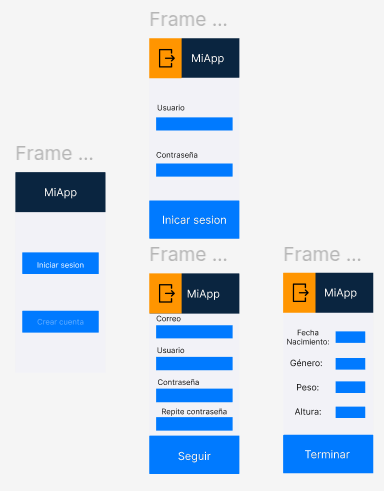
\includegraphics[width=\textwidth]{fotos/Init.png}
    \caption{Pantalla inicial}
    \label{fig:Pantalla inicial}
  \end{minipage}
  \hfill
  \begin{minipage}[b]{0.35\textwidth}
    \centering
    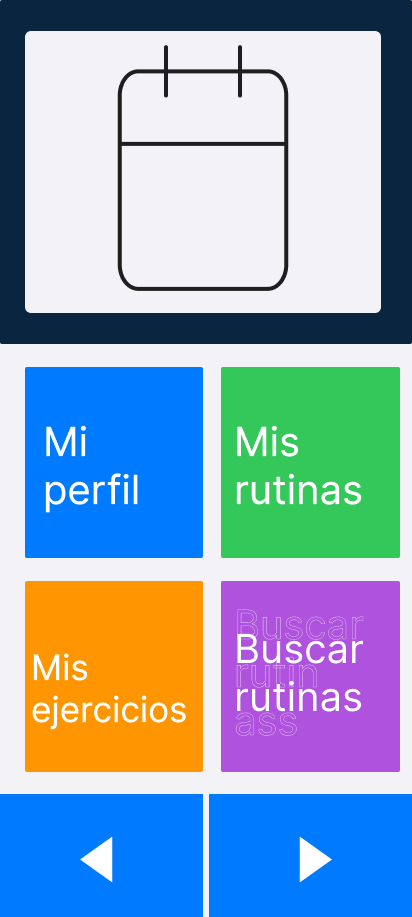
\includegraphics[width=\textwidth]{fotos/MainMenu.png}
    \caption{Menú principal}
    \label{fig:Menu principal}
  \end{minipage}
  \begin{minipage}[b]{0.45\textwidth}
    \centering
    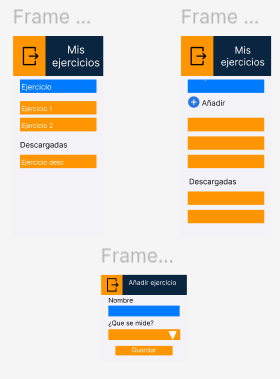
\includegraphics[width=\textwidth]{fotos/ListaEjercicios.png}
    \caption{Lista ejercicios}
    \label{fig:Lista ejercicios}
  \end{minipage}
  \begin{minipage}[b]{0.45\textwidth}
    \centering
    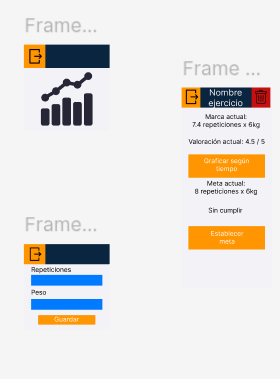
\includegraphics[width=\textwidth]{fotos/DatosEjercicios.png}
    \caption{Datos ejercicios}
    \label{fig:Datos ejericicios}
  \end{minipage}
\end{figure}

\begin{figure}[H]
	\begin{minipage}[b]{0.4\textwidth}
    \centering
    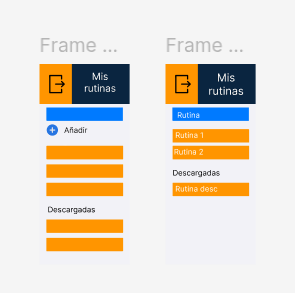
\includegraphics[width=\textwidth]{fotos/ListaRutinas.png}
    \caption{Lista rutinas}
    \label{fig:Lista rutinas}
  \end{minipage}
  \begin{minipage}[b]{0.4\textwidth}
    \centering
    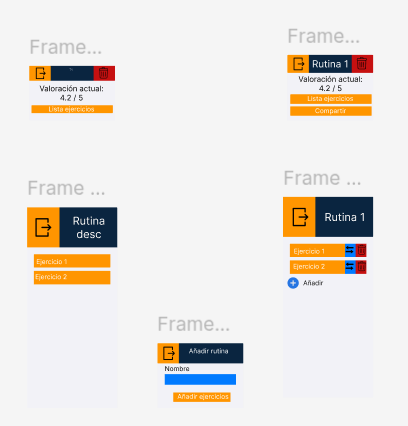
\includegraphics[width=\textwidth]{fotos/DatosRutinas.png}
    \caption{Datos rutinas}
    \label{fig:Datos rutinas}
  \end{minipage}
  \begin{minipage}[b]{0.4\textwidth}
    \centering
    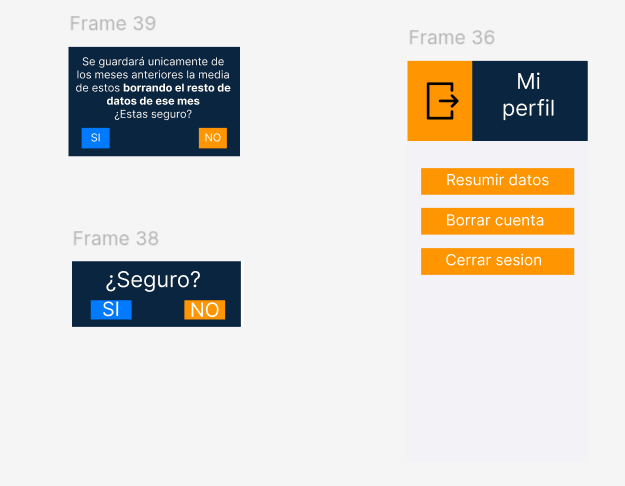
\includegraphics[width=\textwidth]{fotos/MiPerfil.png}
    \caption{Ajustes de perfil}
    \label{fig:Ajustes de perfil}
  \end{minipage}
  \begin{minipage}[b]{0.4\textwidth}
    \centering
    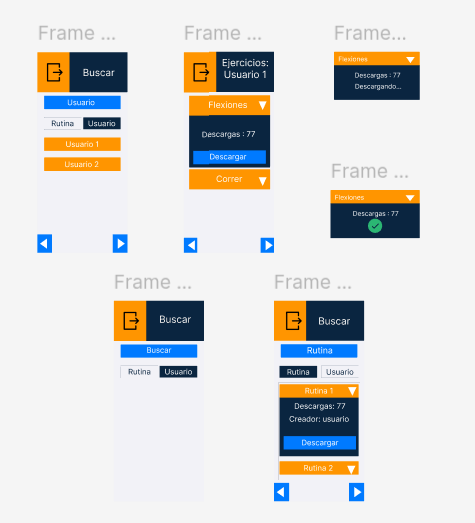
\includegraphics[width=\textwidth]{fotos/DescargarRutinas.png}
    \caption{Descargar rutinas}
    \label{fig:Descargar rutinas}
  \end{minipage}
  \begin{minipage}[b]{0.45\textwidth}
    \centering
    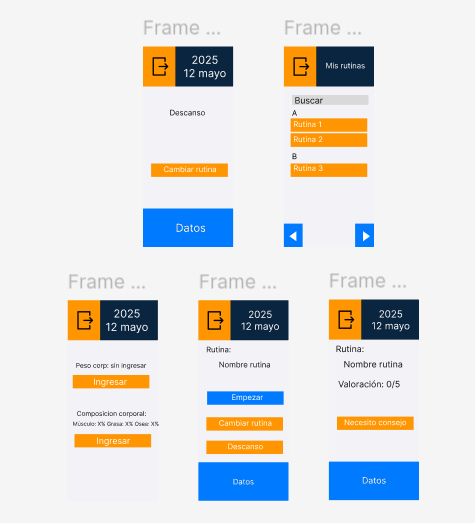
\includegraphics[width=\textwidth]{fotos/SeleccionarEntrenamiento.png}
    \caption{Seleccionar entrenamiento}
    \label{fig:Seleccionar entrenamiento}
  \end{minipage}
\end{figure}
  
\begin{figure}[H]
  \begin{minipage}[b]{0.45\textwidth}
    \centering
    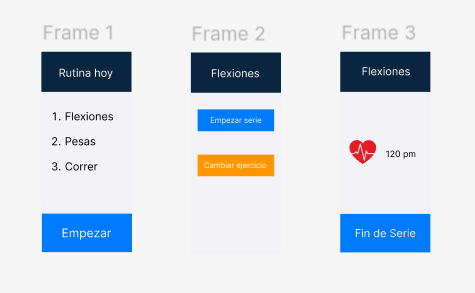
\includegraphics[width=\textwidth]{fotos/FE0.png}
    \caption{Flujo Entrenamiento 0}
    \label{fig:Flujo Entrenamiento 0}
  \end{minipage}
  \begin{minipage}[b]{0.45\textwidth}
    \centering
    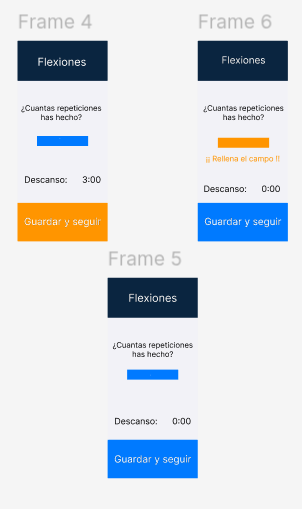
\includegraphics[width=\textwidth]{fotos/FE1.png}
    \caption{Flujo Entrenamiento 1}
    \label{fig:Flujo Entrenamiento 1}
  \end{minipage}
  \begin{minipage}[b]{0.45\textwidth}
    \centering
    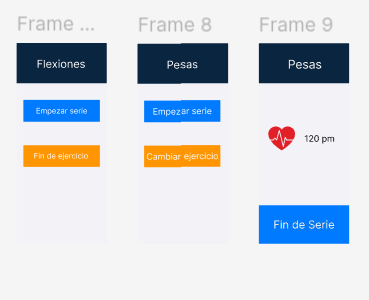
\includegraphics[width=\textwidth]{fotos/FE2.png}
    \caption{Flujo Entrenamiento 2}
    \label{fig:Flujo Entrenamiento 2}
  \end{minipage}
  \begin{minipage}[b]{0.45\textwidth}
    \centering
    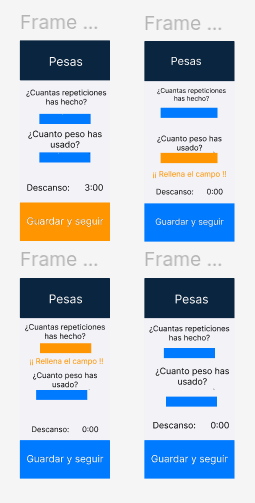
\includegraphics[width=\textwidth]{fotos/FE3.png}
    \caption{Flujo Entrenamiento 3}
    \label{fig:Flujo Entrenamiento 3}
  \end{minipage}
\end{figure}

\begin{figure}[H]
  \begin{minipage}[b]{0.4\textwidth}
    \centering
    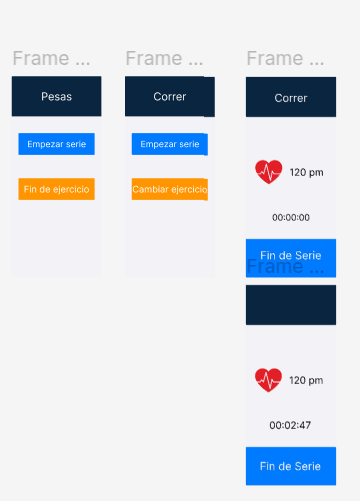
\includegraphics[width=\textwidth]{fotos/FE4.png}
    \caption{Flujo Entrenamiento 4}
    \label{fig:Flujo Entrenamiento 4}
  \end{minipage}
  \begin{minipage}[b]{0.4\textwidth}
    \centering
    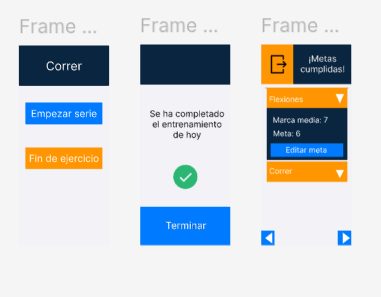
\includegraphics[width=\textwidth]{fotos/FE5.png}
    \caption{Flujo Entrenamiento 5}
    \label{fig:Flujo Entrenamiento 5}
  \end{minipage}
  \begin{minipage}[b]{0.4\textwidth}
    \centering
    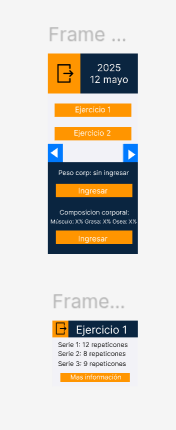
\includegraphics[width=\textwidth]{fotos/FE6.png}
    \caption{Flujo Entrenamiento 6}
    \label{fig:Flujo Entrenamiento 6}
  \end{minipage}
\end{figure}

Estos diseños pueden cambiar y sufrir alteraciones debido a los sprints reviews y correcciones de accesibilidad. De todas formas, cada cambio será informado con su motivo.

\subsubsection*{Sprint Review 0}
Durante esta revisi\'on de sprint se realizaron mejoras de dise\~no, como la incorporaci\'on de iconos en todos los botones para mejorar la accesibilidad. Se revisaron los t\'itulos de las ventanas, cambiando aquellos que no eran lo suficientemente claros.

Adem\'as, se a\~nadieron nuevas historias al \textit{product backlog}:

\begin{itemize}
  \item Copiar rutina
  \item A\~nadir meta por par\'ametro
  \item Solicitar permiso al usuario antes de enviar datos a la IA
  \item Enviar datos del entrenamiento actual y anteriores a la IA
  \item Conectar/Desconectar con la IA
\end{itemize}

\subsection*{Iteraci\'on 1}
Al inicio de esta iteraci\'on detect\'e la ausencia de historias para el dise\~no de diagramas de la app y la base de datos. Por ello, se a\~nadi\'o la siguiente historia:

\begin{description}
  \item[\textbf{SCRUM-26}] Dise\~nar las tablas de la base de datos
\end{description}

\begin{figure}[h!]
  \centering
  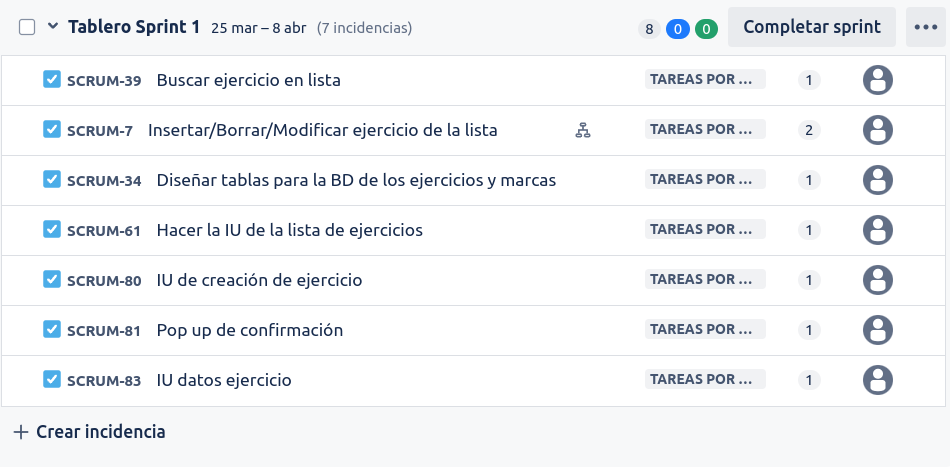
\includegraphics[width=0.7\textwidth]{fotos/PreSrprint1.png}
  \caption{Planificaci\'on Sprint 1}
  \label{fig:pre_sprint1}
\end{figure}

\begin{figure}[h!]
  \centering
  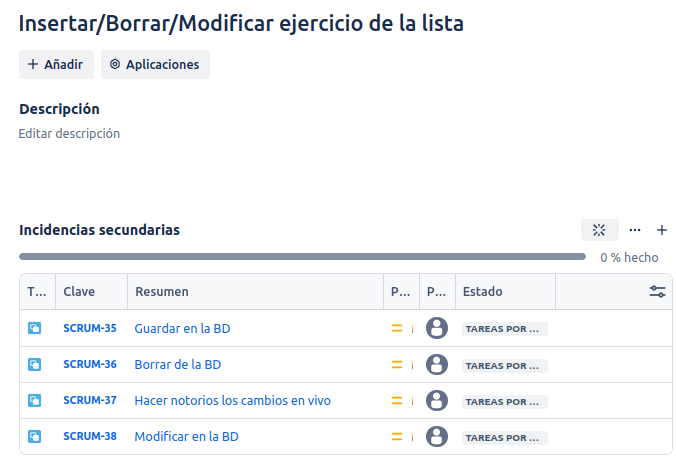
\includegraphics[width=0.7\textwidth]{fotos/SubListPre1.png}
  \caption{Subtareas Sprint 1}
  \label{fig:sublist_pre1}
\end{figure}

Durante esta iteraci\'on me familiaric\'e con Flutter y sus herramientas, como la base de datos local \textit{SQLite}.

\subsubsection*{SQLite}
Es una base de datos ligera, autocontenida y de c\'odigo abierto. Usa el mismo lenguaje de consultas que SQL, lo que la hace ideal para la app. Adem\'as, permite transportar toda la BD en un \textit{.db}, lo cual puede facilitar funcionalidades como copias de seguridad descargables desde la nube.

\subsubsection*{Sprint Review 1}
Las primeras iteraciones tienden a ser m\'as lentas debido a la fase inicial del desarrollo. No se complet\'o la totalidad del sprint; qued\'o pendiente la subtarea de modificar ejercicio en la base de datos. Aun as\'i, las expectativas son positivas, ya que se espera un aumento en la velocidad de desarrollo. No obstante, en lo que se lleva  desarrollado han aparecido pocas problemáticas

\begin{figure}[h!]
  \centering
  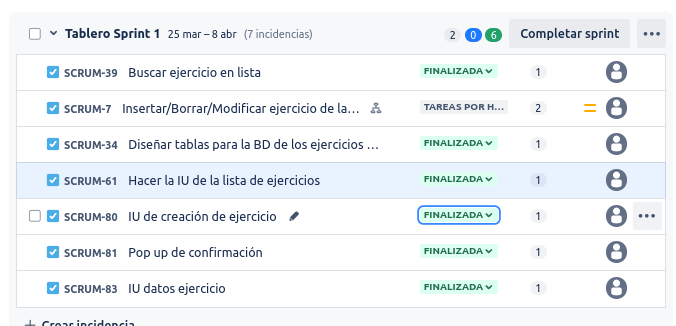
\includegraphics[width=0.7\textwidth]{fotos/PostSprint1.png}
  \caption{Fin Sprint 1}
  \label{fig:post_sprint1}
\end{figure}

\begin{figure}[h!]
  \centering
  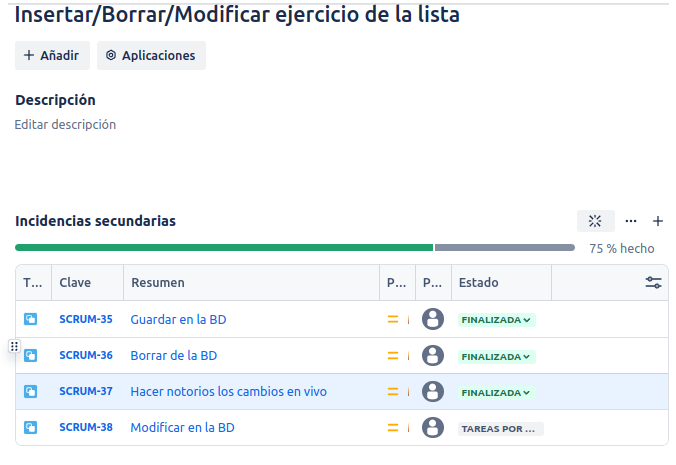
\includegraphics[width=0.7\textwidth]{fotos/SubListPost1.png}
  \caption{Subtareas completadas Sprint 1}
  \label{fig:sublist_post1}
\end{figure}

\begin{figure}[h!]
  \centering
  \begin{minipage}[b]{0.45\textwidth}
    \centering
    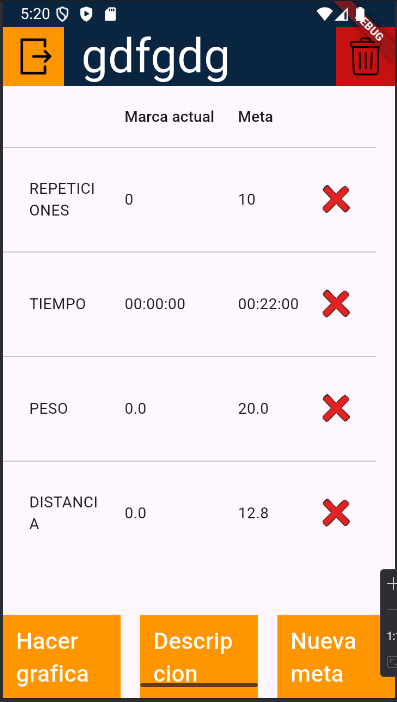
\includegraphics[width=\textwidth]{fotos/ejerciciosNueva.png}
    \caption{Pantalla nueva}
    \label{fig:pantalla_nueva}
  \end{minipage}
  \hfill
  \begin{minipage}[b]{0.45\textwidth}
    \centering
    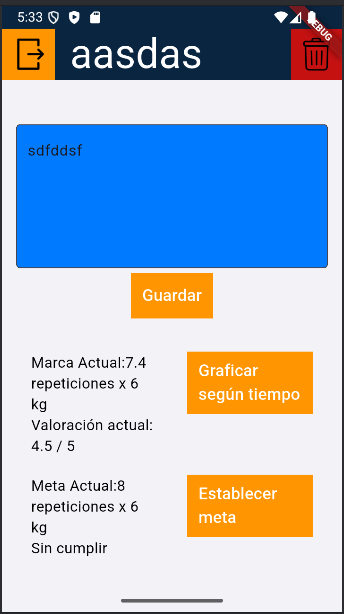
\includegraphics[width=\textwidth]{fotos/ejerciciosVieja.png}
    \caption{Pantalla antigua}
    \label{fig:pantalla_vieja}
  \end{minipage}
  \caption{Comparaci\'on entre la pantalla nueva y la anterior}
  \label{fig:comparacion_pantallas}
\end{figure}

\subsection*{Iteraci\'on 2}
Esta iteraci\'on se centr\'o en el desarrollo del sistema de sesiones, la API de la aplicaci\'on, el backend b\'asico del servidor y la secci\'on de rutinas.

\begin{figure}[h!]
  \centering
  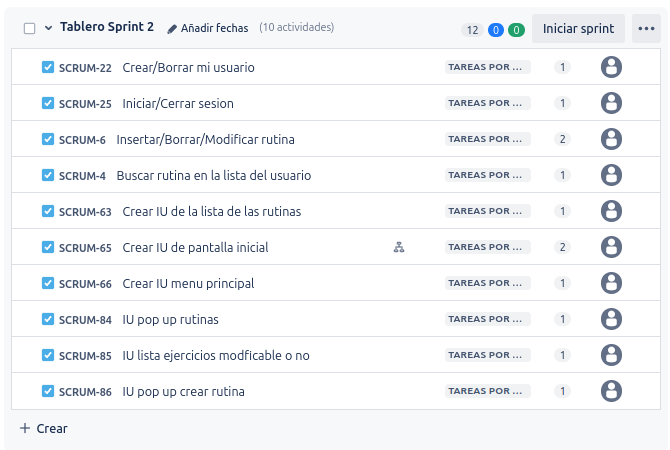
\includegraphics[width=0.7\textwidth]{fotos/PreSprint2.png}
  \caption{Planificaci\'on Sprint 2}
  \label{fig:pre_sprint2}
\end{figure}

\begin{figure}[h!]
  \centering
  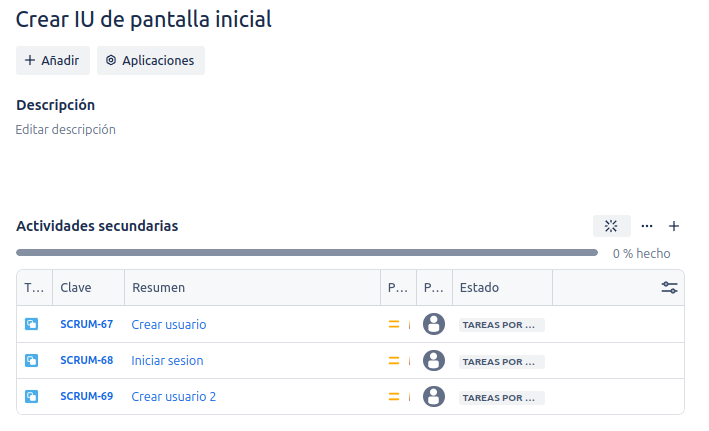
\includegraphics[width=0.7\textwidth]{fotos/SubListPre2.png}
  \caption{Subtareas Sprint 2}
  \label{fig:sublist_pre2}
\end{figure}

\subsubsection*{Sistema de sesiones}
Se implement\'o un sistema de autenticaci\'on basado en tokens. Cuando el usuario verifica su identidad, recibe un token que se guarda en el dispositivo y se usa para validar el acceso posterior. Esto evita que usuarios no autorizados suban contenido haci\'endose pasar por otros.

El backend est\'a desarrollado en \textit{Node.js} y utiliza una base de datos SQL para gestionar las contrase\~nas de los usuarios. Este mismo backend se usar\'a para las funcionalidades de las siguientes iteraciones.

\subsubsection*{API de la app}
La comunicaci\'on entre la app y el servidor se realiza mediante peticiones HTTP. En el futuro, estas podr\'an migrarse a HTTPS para proteger operaciones sensibles. Por ahora se mantiene HTTP para facilitar el depurado.

\subsubsection*{Cambios importantes}
Se redise\~n\'o la implementaci\'on de las pantallas con listas. En lugar de una \'unica clase con condiciones para la visibilidad de elementos, se opt\'o por crear clases espec\'ificas para cada tipo de lista.

\textbf{Ventaja:} El c\'odigo es m\'as limpio, escalable y modular. Si hay que modificar un tipo de lista, los dem\'as no se ven afectados.

\subsubsection*{Sprint Review 2}
Se sugirieron mejoras menores como el ajuste de tama\~nos e iconos en los botones de la secci\'on de creaci\'on de rutinas.

Tambi\'en se modific\'o la funcionalidad de compartir rutinas. Ahora todas son modificables, eliminando la distinci\'on entre rutinas descargadas (antes no modificables) y creadas (modificables). Esto mejora la experiencia del usuario: si desea volver a una rutina original, simplemente la puede volver a buscar y descargar.

\begin{figure}[h!]
  \centering
  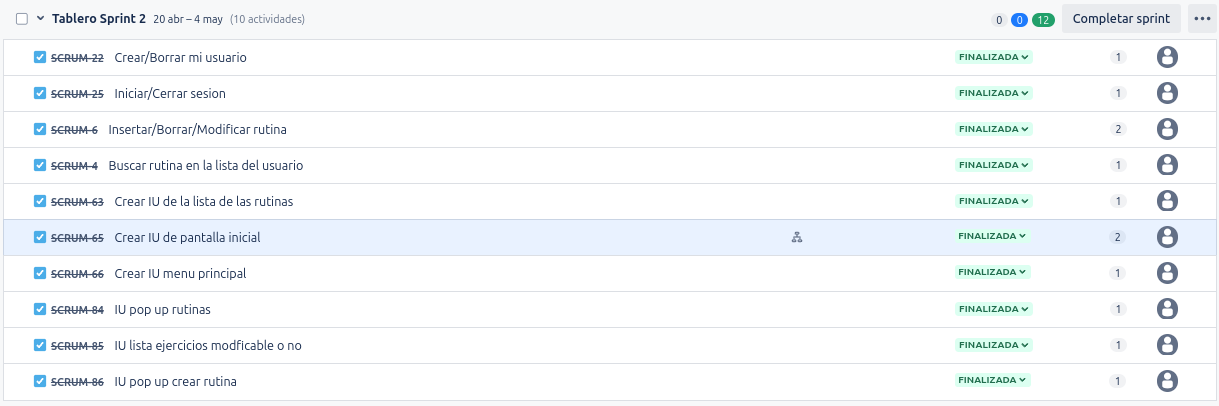
\includegraphics[width=0.7\textwidth]{fotos/PostSprint2.png}
  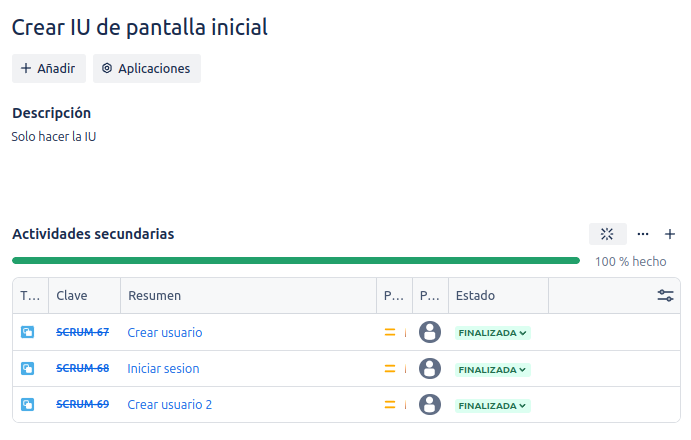
\includegraphics[width=0.7\textwidth]{fotos/SubListPost2.png}
  \caption{Fin Sprint 2 y subtareas}
  \label{fig:post_sprint2}
\end{figure}


\subsection*{Iteraci\'on 3}
Esta iteraci\'on se centr\'o en desarrollar la funcionalidad para compartir rutinas entre usuarios, incluyendo la subida, visualizaci\'on y descarga de rutinas. Adem\'as, se comenz\'o a implementar la funcionalidad de resumen de datos para optimizar el uso de la memoria local.

\begin{figure}[h!]
  \centering
  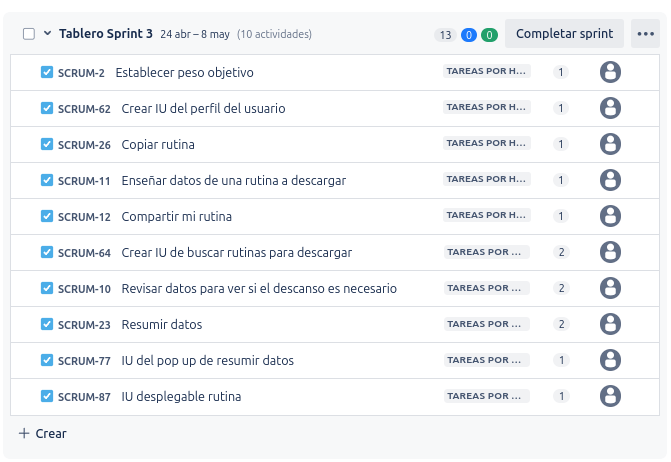
\includegraphics[width=0.7\textwidth]{fotos/PreSprint3.png}
  \caption{Planificaci\'on Sprint 3}
  \label{fig:pre_sprint3}
\end{figure}

\subsubsection*{Peso objetivo}
El peso objetivo es una meta que define el usuario y se almacena en memoria. Esta meta se representar\'a en la gr\'afica de evoluci\'on del peso del usuario, y se generar\'a una alerta cuando dicha meta sea alcanzada. La visualizaci\'on a\'un no ha sido implementada completamente.

\subsubsection*{Cambios durante el desarrollo}
Durante esta iteraci\'on surgieron cambios en la forma de visualizar y gestionar las rutinas compartidas y almacenadas:

\begin{itemize}
  \item Ahora, al descargar una rutina, se a\~nade el nombre del creador al nombre de la rutina, facilitando la distinci\'on entre rutinas propias y descargadas.
  \item Cuando hay conflicto de nombres al crear una rutina, se genera un nombre alternativo del tipo \texttt{Nombre(n)}, siendo \texttt{n} un n\'umero incremental.
  \item Se ha implementado un selector entre ``Mis rutinas'' y ``Compartidas'' para facilitar la visualizaci\'on de las rutinas subidas a la nube por el usuario.
  \item Se reemplaz\'o el filtro integrado en la ventana de b\'usqueda por un selector emergente que permite buscar rutinas por nombre o por nombre de usuario.
  \item La interfaz de descarga y visualizaci\'on de rutinas ahora es un cuadro emergente (pop-up) en lugar de un desplegable.
\end{itemize}

\subsubsection*{Imprevistos y problemas en el desarrollo}
Se identificaron dos errores principales de planificaci\'on:

\begin{description}
  \item[Error 1:] Se planific\'o implementar la funcionalidad de resumir datos sin haber completado la obtenci\'on de datos. \\ \textbf{Soluci\'on:} Replanificar los sprints.
  \item[Error 2:] Se subestim\'o la complejidad del sistema de rutinas compartidas, especialmente en la resoluci\'on de conflictos de nombres. \\ \textbf{Soluci\'on:} Aplicar nombres combinados (nombre + creador + copia) en memoria local e identificadores \textit{autoincrementales} en la nube.
\end{description}

\subsubsection*{Valor a\~nadido a la app}
Los imprevistos y problemas surgidos durante el desarrollo han permitido detectar \textit{bugs}, errores de dise\~no y carencias funcionales que de otro modo podr\'ian haber pasado desapercibidos. Gracias a ello, se han podido proponer nuevas funcionalidades y mejorar las ya existentes, lo cual contribuye significativamente a aumentar la calidad global de la aplicaci\'on.

Algunas de las funcionalidades propuestas como mejora son:

\begin{itemize}
  \item Verificar el token del usuario antes de permitir la subida de rutinas, para evitar plagios.
  \item Al seleccionar la opci\'on de borrar usuario del dispositivo, eliminar tambi\'en la base de datos local asociada.
  \item Crear una base de datos local independiente para cada nuevo usuario creado en un dispositivo.
  \item Posibilidad de editar el nombre de una rutina.
  \item Marcar los ejercicios eliminados con una \textit{flag}, para evitar que se inicien rutinas que los contengan.
  \item Marcar a los usuarios permanentemente eliminados con una \textit{flag}, para proceder a eliminarlos en los dispositvos.
\end{itemize}

Estas funcionalidades est\'an pensadas para aportar mayor \textbf{seguridad}, \textbf{integridad} y \textbf{calidad} al producto final.

\subsubsection{Base de datos del backend}
La base de datos utilizada en el backend está basada en \textit{MySQL}. En ella se almacenan los usuarios junto con sus contraseñas, así como los ejercicios y las rutinas. Las rutinas están vinculadas al usuario que las creó, y los ejercicios se asocian a las rutinas a las que pertenecen. Si un usuario decide eliminar su cuenta de forma permanente, las rutinas y ejercicios relacionados se eliminarán en cascada.

Al descargar una rutina, los ejercicios asociados se guardan en la memoria local del usuario como si fueran de su propiedad. Es decir, el usuario puede modificarlos libremente sin restricciones.

\subsubsection{Sprint Review 3}

	
	\newpage
	\printbibliography

	
\end{document}

